\begin{example2}[\quad \large Sorrendi logikai hálózatok 3.]

D tároló(k) és NAND kapu(k) felhasználásával valósítsa meg a következő funkciót:
A CLK órajel felfutó élénél a két Q kimenet rendre az alábbi értékeket veszi fel: 00, 01, 10, 11, 00…
\end{example2}

A feladatban egy sorrendi logikai hálózatot kell terveznünk. Először is, nézzük meg, hogy hány állapotváltozóra, vagyis memóriaelemre van szükségünk. Mivel 2 biten kell adatot tárolnunk, mindegyik bit egy-egy állapotváltozó, így mindegyik bit tárolására szükségünk van. \\ \\
\underline{Tehát a feladat megoldása két D flip-flopot fog igénybe venni.} \\


Második lépésben vegyük fel a rendszer állapotdiagrammját. Az állapotdiagramm egy irányított gráf, melynek csúcsai a rendszer állapotait, élei pedig az azok közti átmenetet jelképezik. Ebben az esetben a következőképpen néz ki:

\begin{figure}{}
    \centering
    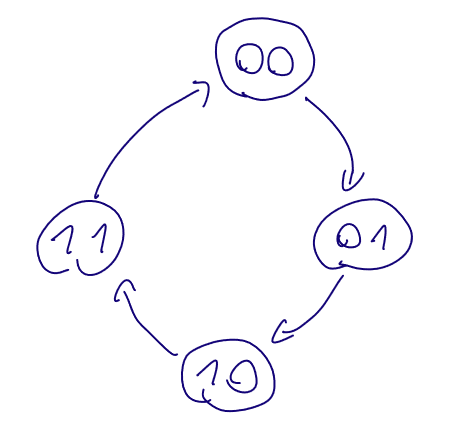
\includegraphics[width=0.24\textwidth]{Figures//tmp/sd_counter.png}
    \caption{Enter Caption}
    \label{fig:enter-label}
\end{figure}

Mivel csak egy irányba kell számolnunk, ezért csak egyfajta utat kell feltüntetnünk a gráfon. Az állapotok elnevezésénél a kimenet értékét használtuk, ezzel gyakorlatileg elvégeztük az \textbf{állapot kódolást} is, hiszen ha a bináris szám bitjeit $q_0$-nak és $q_1$-nek nevezzük, ahol $q_0$ a legalacsonyabb helyiérték, úgy ezekenk a számoknak megfeleltethetjük a D flip-flopok Q kimeneteit.

\begin{equation}
\begin{aligned}{}
    q_0 &= Q_0 \\
    q_1 &= Q_1 \\
\end{aligned}
\end{equation}

Harmadik lépésben nézzük meg, hogy a következő állapotot milyen kombinációs logikai hálózattal tudjuk előállítani. Ehhez bemenetként ebben a feladatban csak az aktuális állapotok szolgálnak. (Ha pl. a feladat része lenne, hogy lehessen váltani a számláló irányát, úgy egy DIR bemenetünk is megjelenne, amely független az aktuális állapotoktól, és az állapotdiagrammot is ki kéne egészítenünk egy másik iránnyal.) \\

A logikai hálózat meghatározásához az állapottáblát kell felírnunk:

\begin{figure}[h!]
    \centering
    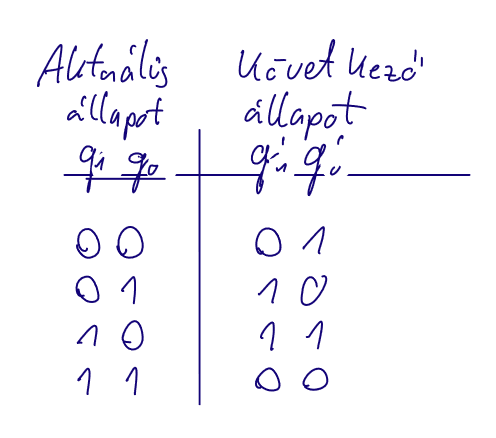
\includegraphics[width=0.5\linewidth]{31_allapottabla.png}
    \caption{Állapottábla}
    \label{fig:enter-label}
\end{figure}

Az állapottáblából kiolvashatjuk az egyes állapotvátozók következő állapotát meghatározó igazságtáblát.
\begin{figure}[h!]
        \centering
        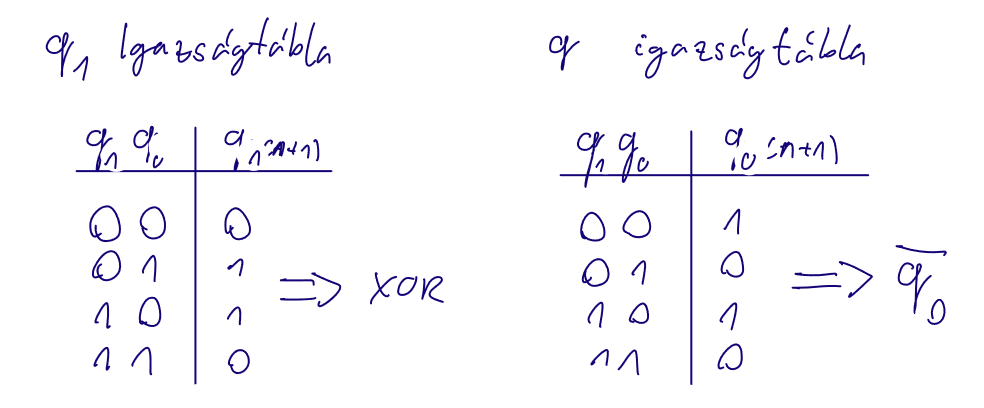
\includegraphics[width=0.75\linewidth]{Figures//tmp/31_igazsagtabla.png}
        \caption{Igazságtábla}
        \label{fig:enter-label}
    \end{figure}
    
Ezekből az igazságtáblákból látszik, hogy:

\begin{equation}
\begin{aligned}{}
    q_{0(n+1)} &= \bar{q_0} \\
    q_{1(n+1)} &= q_0 \oplus q_1 \\
\end{aligned}
\end{equation}

Innen pedig a hálózat már egyszerűen felrajzolható:
\begin{figure}[h!]

    \centering
    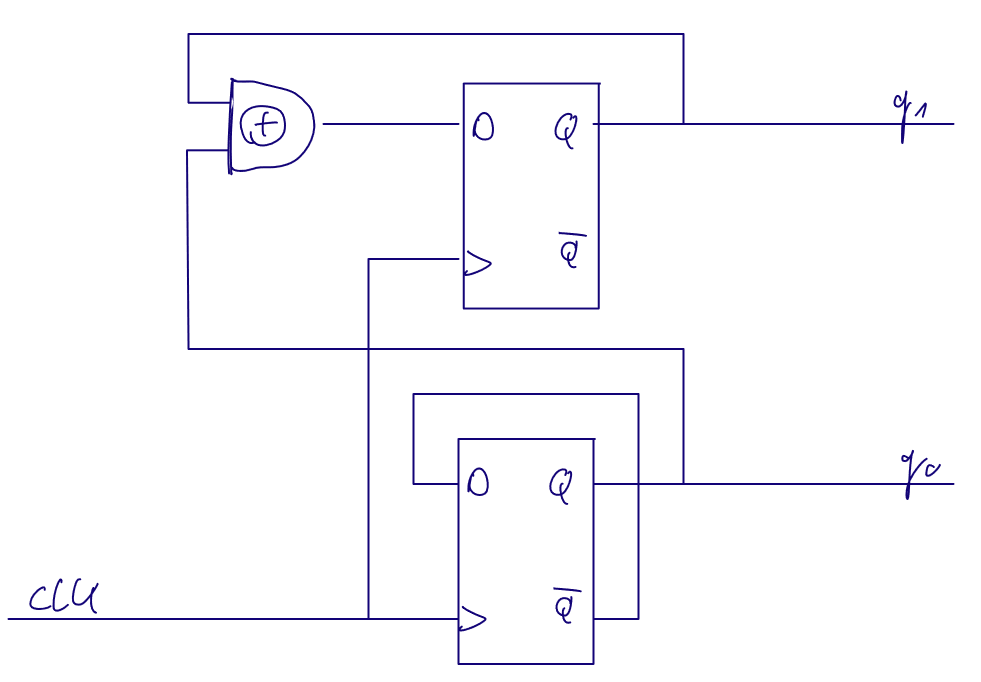
\includegraphics[width=0.75\linewidth]{Figures//tmp/31_schematic.png}
    \caption{2 bites számláló kacspolási rajza}
    \label{fig:enter-label}
\end{figure}
